


\thispagestyle{empty}
\mbox{}
\vfill
\begin{center}
    \textit{This page is left intentionally blank.}
\end{center}
\vfill
\newpage
\noindent


\begin{multicols}{2}

\noindent
---\textbf{System}---\textbf{Threads:} Hardware threads (CPU cores) each
may run one software thread (program) at a time. Switching,
between threads is context switching (overhead). E.g.,
Go manages internal thread pools, offering it to the OS,
reducing overhead.
\textbf{Thread Comm:} Inter-process communication (IPC), 
threads communicate via shared memory (e.g., channels, pipes, virtual memory).
\textbf{Conc. \& Parrelism:} Concurrency shuffles tasks,
parallelism runs tasks simultaneously (threads).
\textbf{Dist. Conn:} A client connects to a server (client-server model), a TCP conn. (FIFO)
secures the line, the RPC (remote procedure call) abstracts
dist. communication.
\textbf{Races \& Deadlocks:} Data race, two threads manipulating shared data (reads-onlys are fine).
\textbf{Mutexes:} Placing locks around shared data, stopping concurrent access.
\textbf{RPC Failure Models:} At-least-once, client retries until a response is received.
Rads are fine, writes cause race conditions. At-most-once, server handles dupes, clients
send unique IDs (cached responses). Exactly-once, both at-least-once and at-most-once.
\textbf{(a)sync:} Asynchronous, non-blocking, no waiting for a response. Synchronous, blocking, waiting for a response.
\textbf{(un)buffered-channers:} Unbuffered, sender waits for receiver on some thread to receive message. Buffered, sender sends message(s) to a buffer, takes one at a time.
\textbf{Task, Data, Pipeline Parallelism:} Task, same data, different tasks. Data, same task, different data. Pipeline, task split into dependent stages, independent stages run in parallel.
\textbf{Time Accr:} Physical clocks drift due to hardware limitations. Atomic clocks, have insignificant drift. NTP (network time protocol), 
utilizes GPS satellites to sync time, to a ground truth clocks, which propagates time to other systems.
---\textbf{Logical Time}---\textbf{Lamport Clocks:} 
Lamport Clocks, $(t_p, p)$, $t_p$ time of process $p$, monotonically increases for each event/send (Total Ordering). 
Receivers $q$ resolve time differences, $t_q = max((t_p+1), t_q)$ (send vs. local time). Given 
two events $a$ \& $b$, timestamps $t(a)$ \& $t(b)$, with $r$ trace: $a\to_r b \implies t(a) < t(b)$ (causal ordering);
$t(a) \geq t(b) \implies a \not\to_r b$ (concurrent); $(t(a) = t(b) \land a\gg b) \implies a \to_r b$, s.t., ($\gg$) rep. process order.
\textbf{Non-causal:} $(a\ll b):= (a \not\to_r b) \land (b\not\to_r a)$ (concurrent).
\textbf{Vector Clocks:} Operate as an array of Lamport clocks, index is process $p_i$, and value is $t_{p_i}$ (time); However, sends do not increment $t_{p_i}$.
Given timestamps $a$ \& $b$, if all indexes in $a$ are larger than $b$, $a\to_r b$. If some in $a$ are larger than $b$, vice versa, $a<>b$ (non-comparable, concurrent, partial ordering).

\noindent
TaskPar. DataPar. PipePar. Lamp.Clock:
\noindent
\rule{\linewidth}{0.4pt}\\
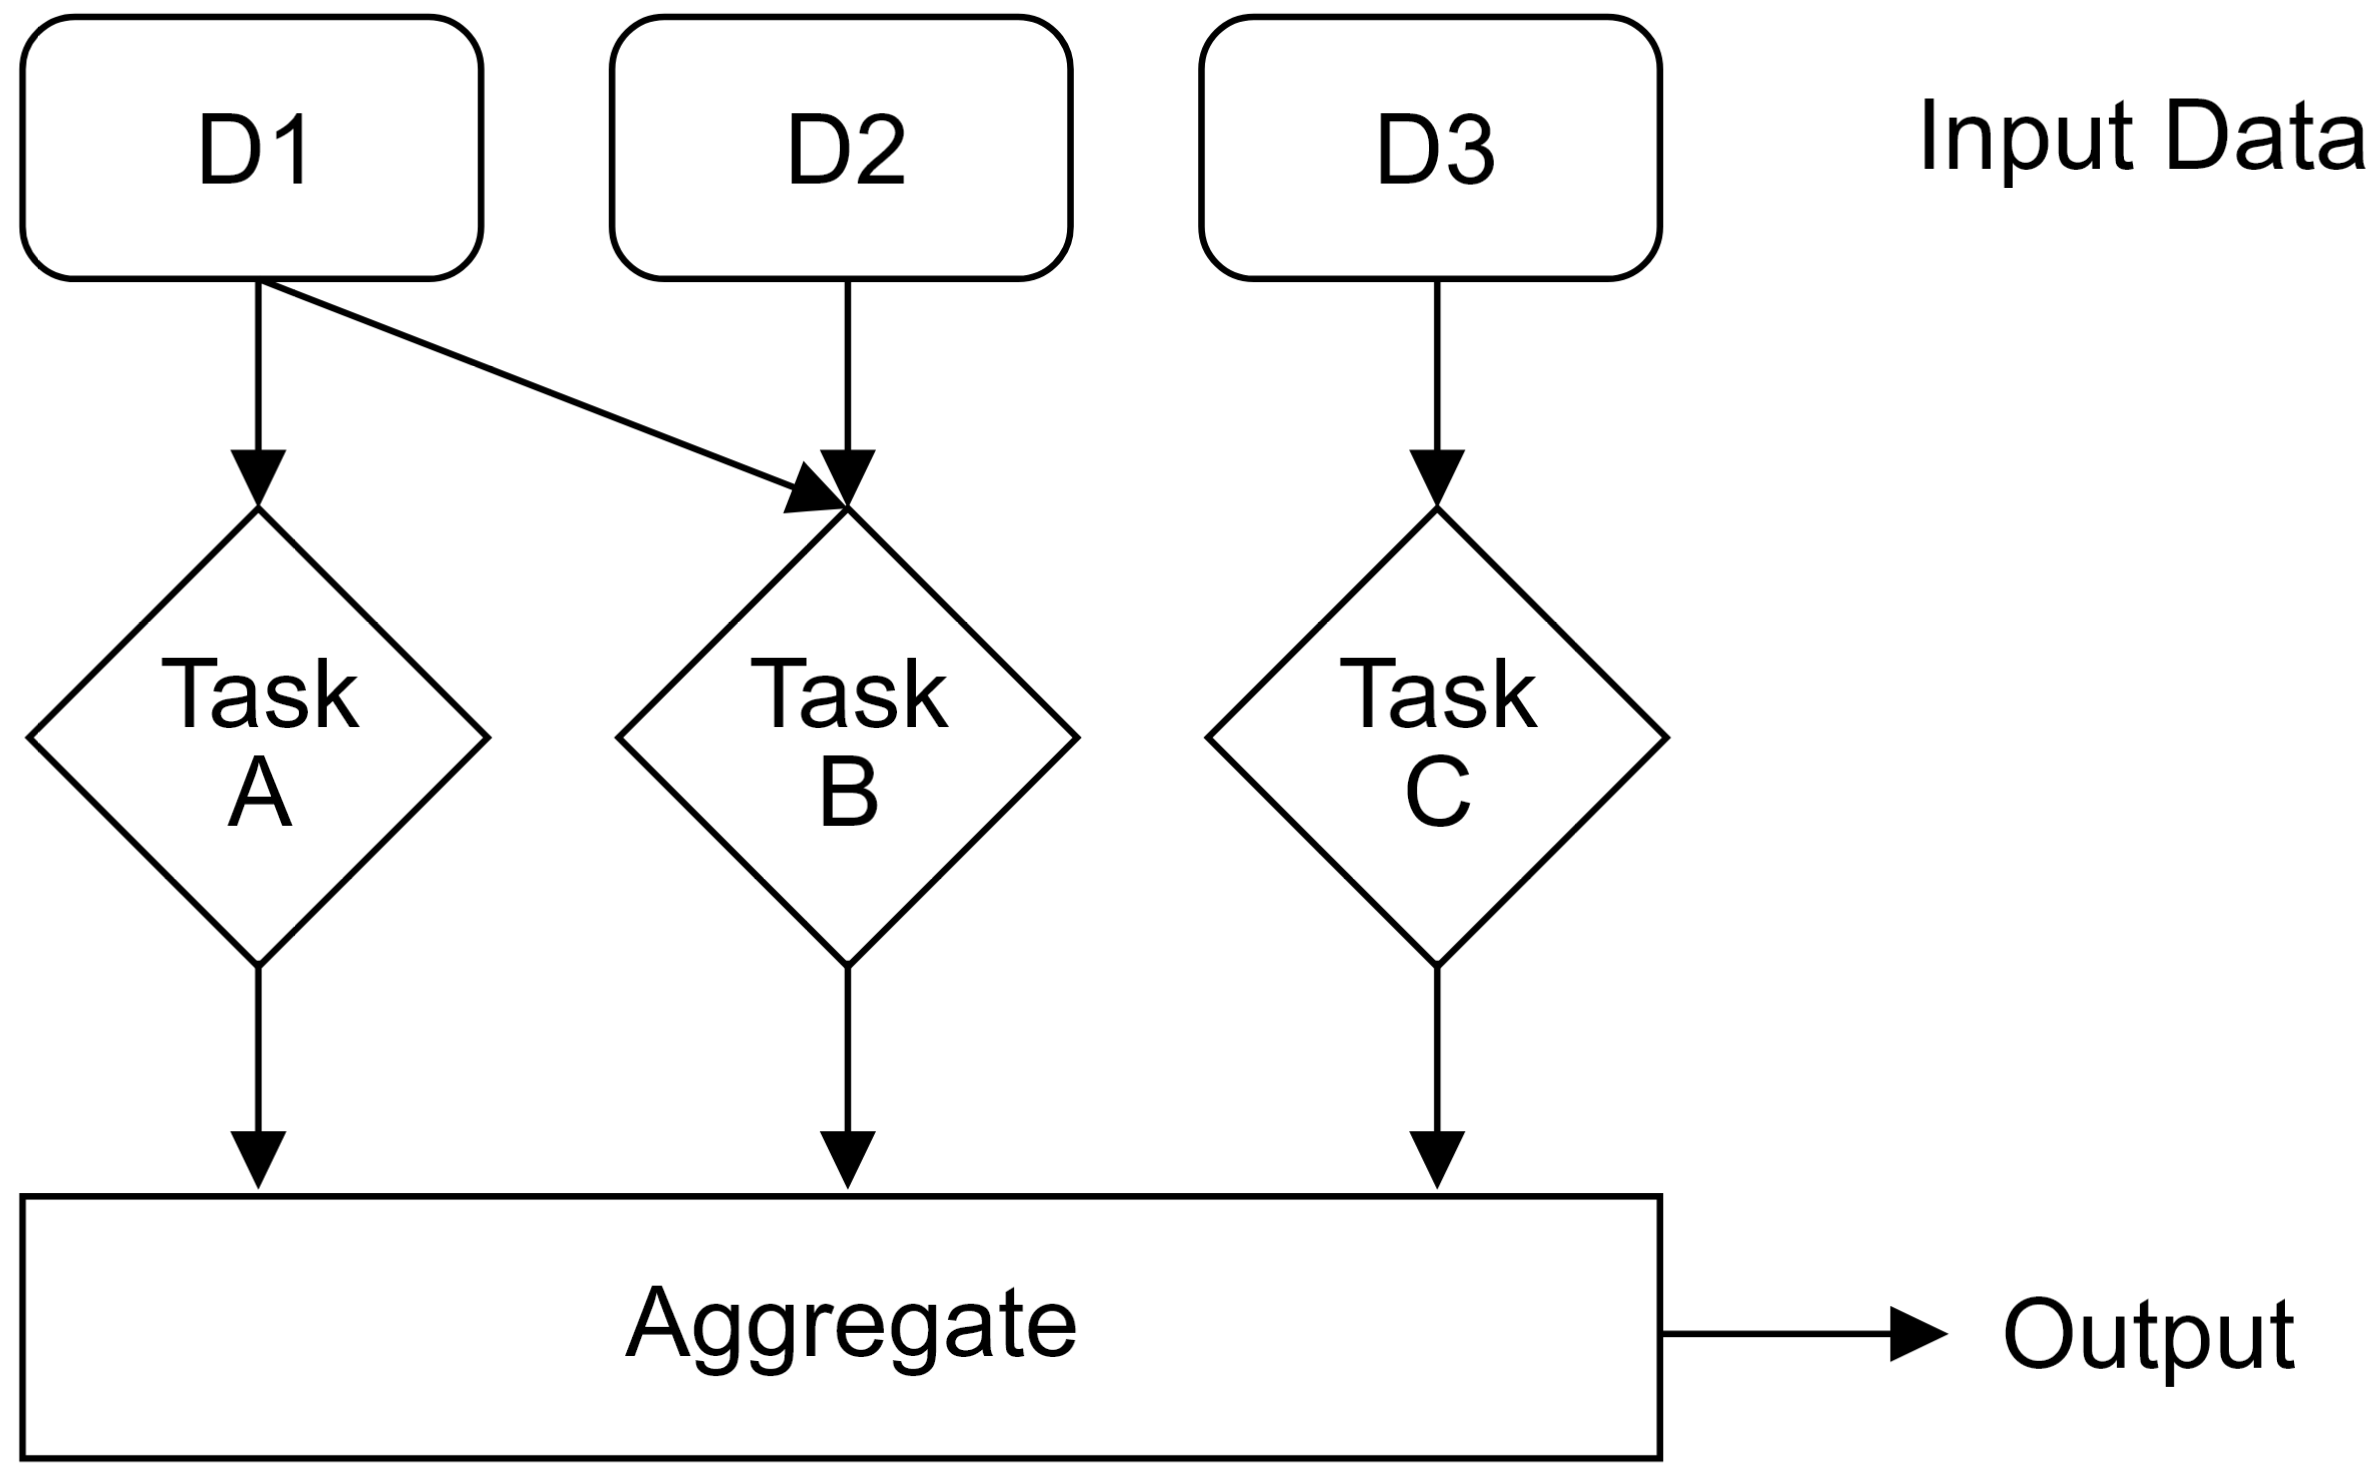
\includegraphics[width=.7\linewidth]{./Sections/rpc_2/tpar.png}\\
\noindent
\rule{\linewidth}{0.4pt}\\
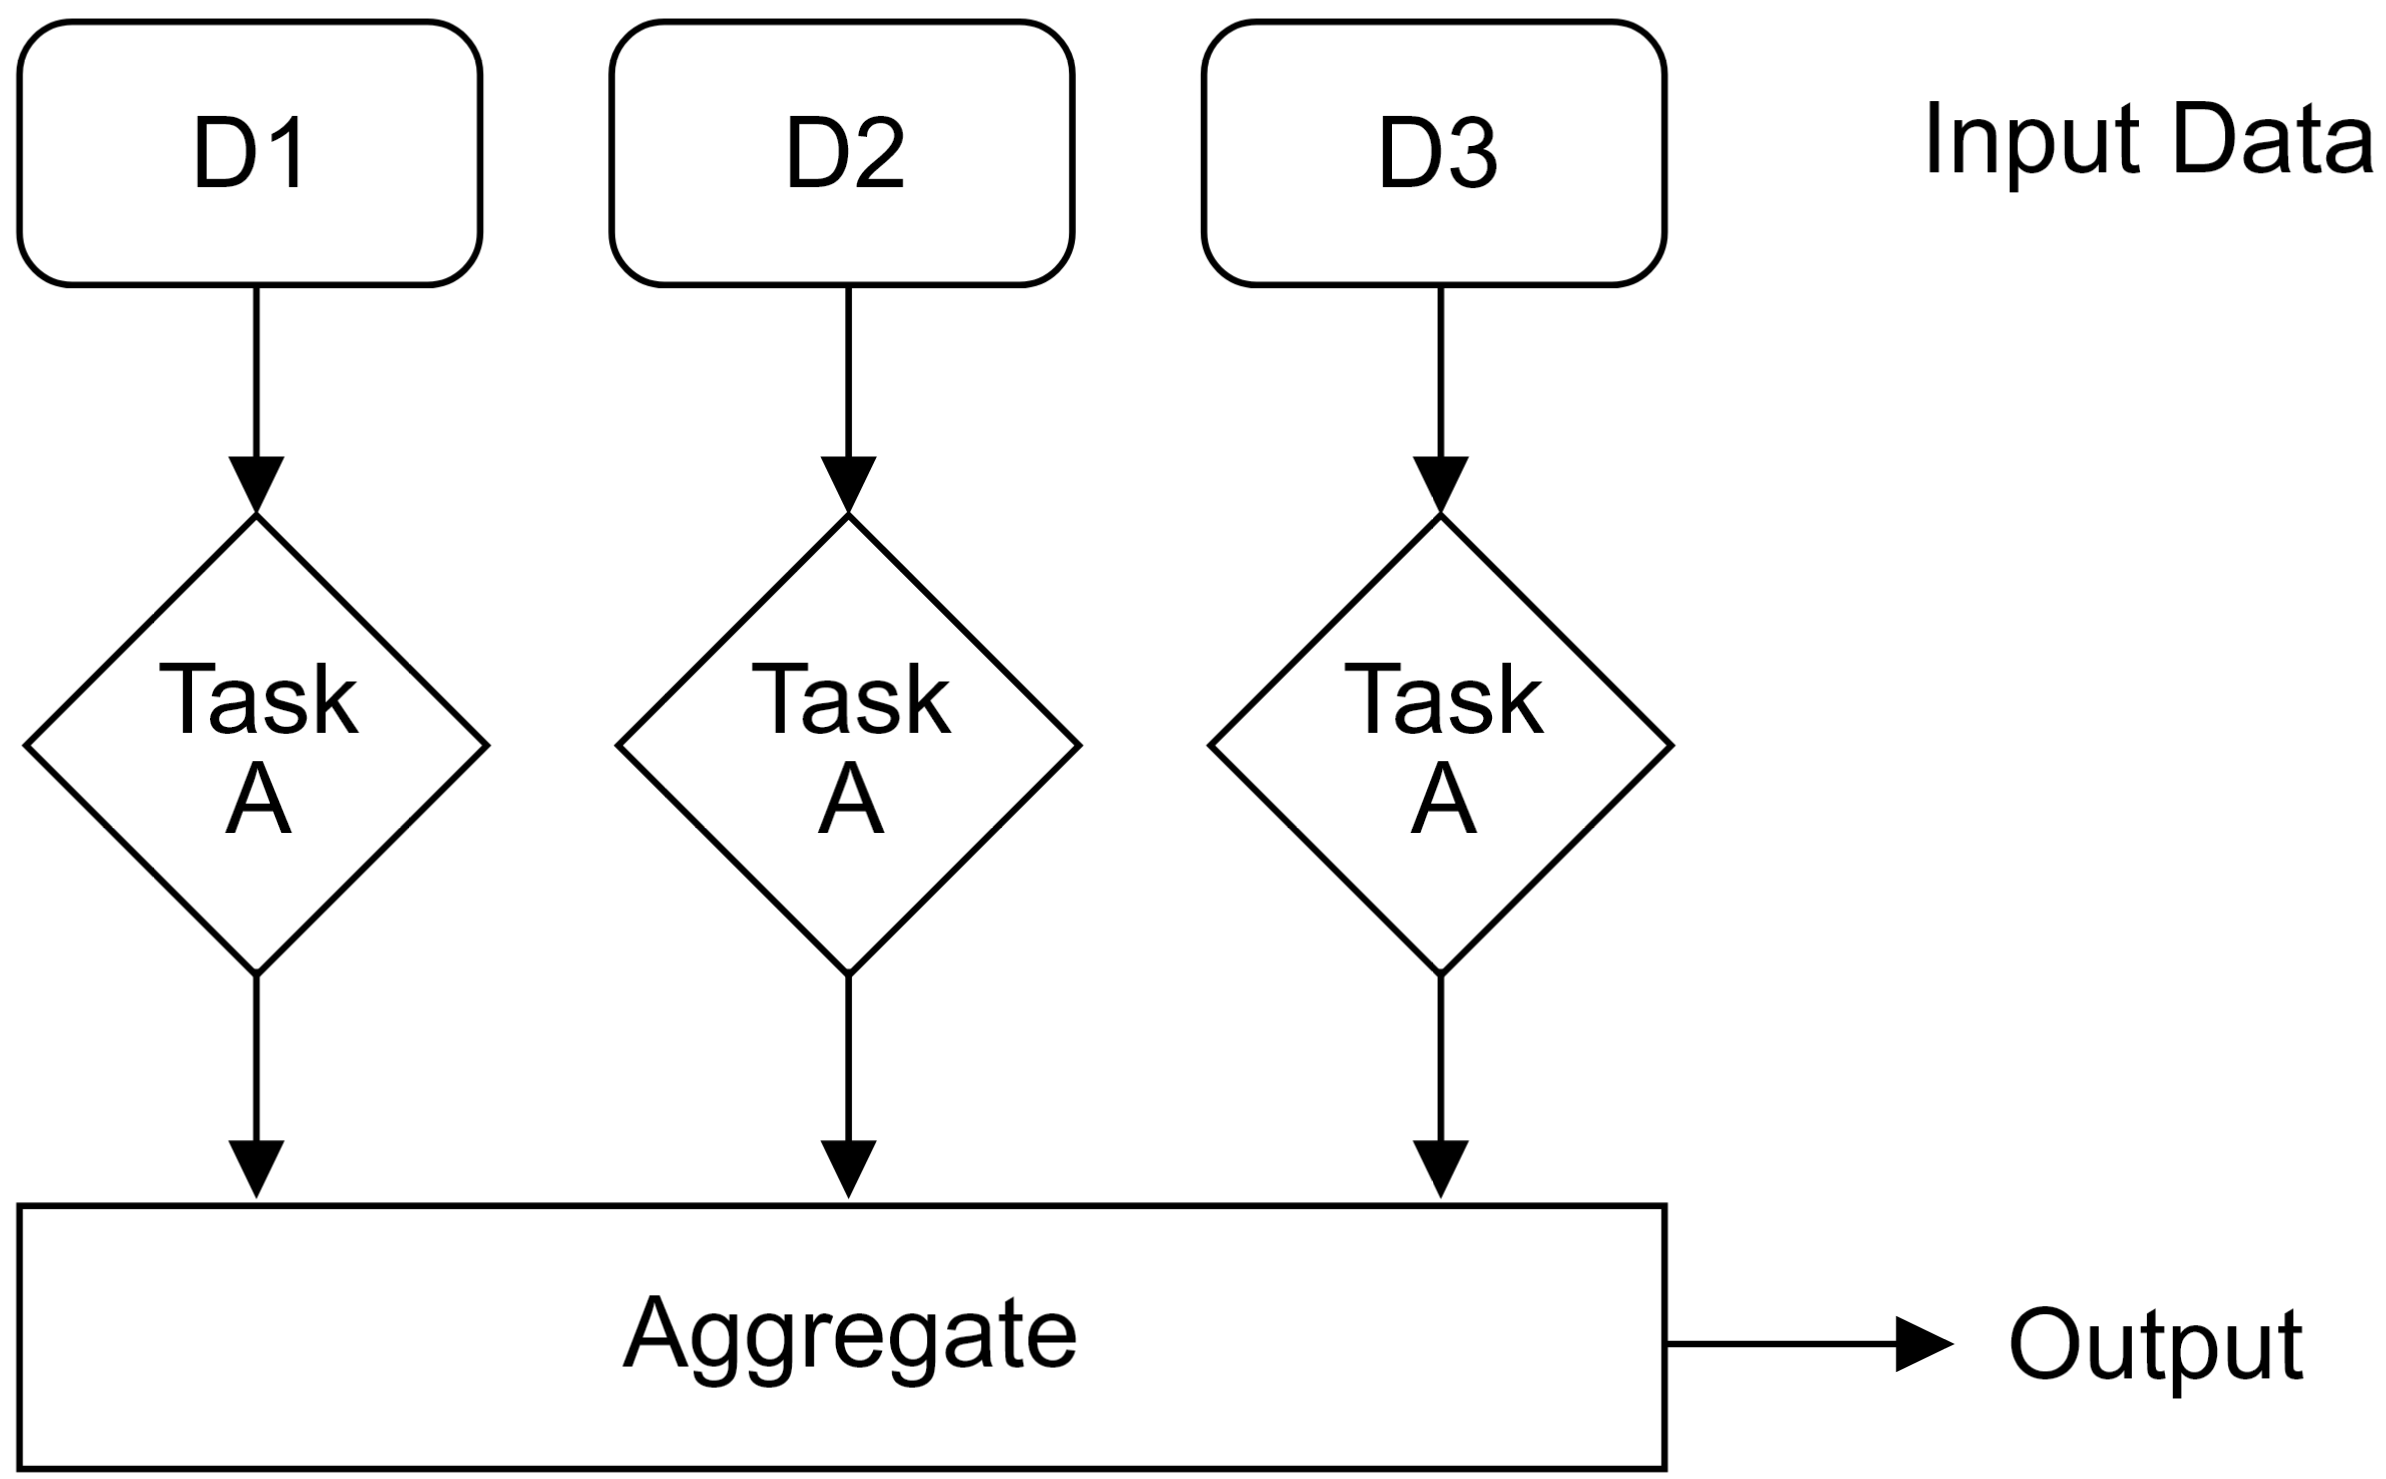
\includegraphics[width=.7\linewidth]{./Sections/rpc_2/dpar.png}\\
\noindent
\rule{\linewidth}{0.4pt}\\
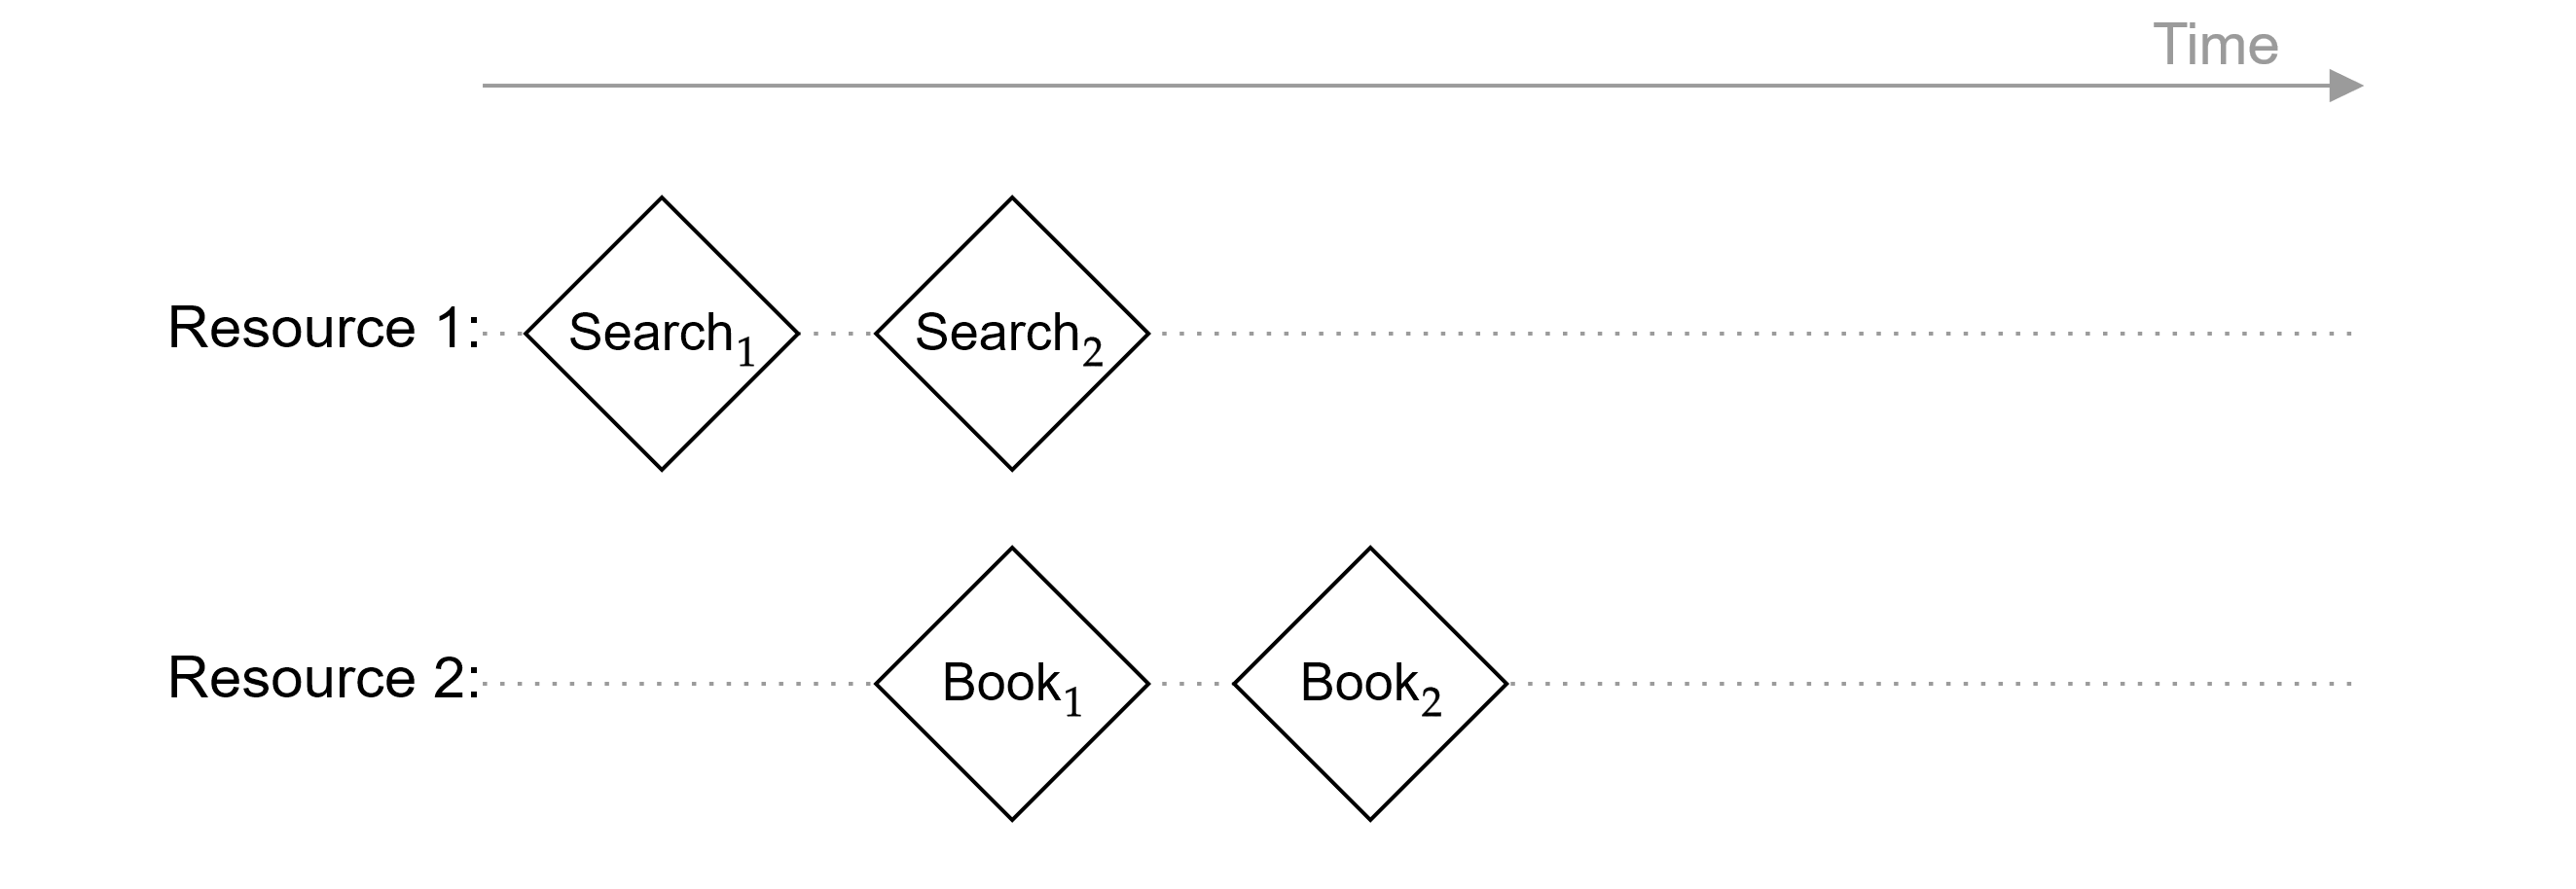
\includegraphics[width=\linewidth]{./Sections/rpc_2/ppar_2.png}
\noindent
\rule{\linewidth}{0.4pt}\\
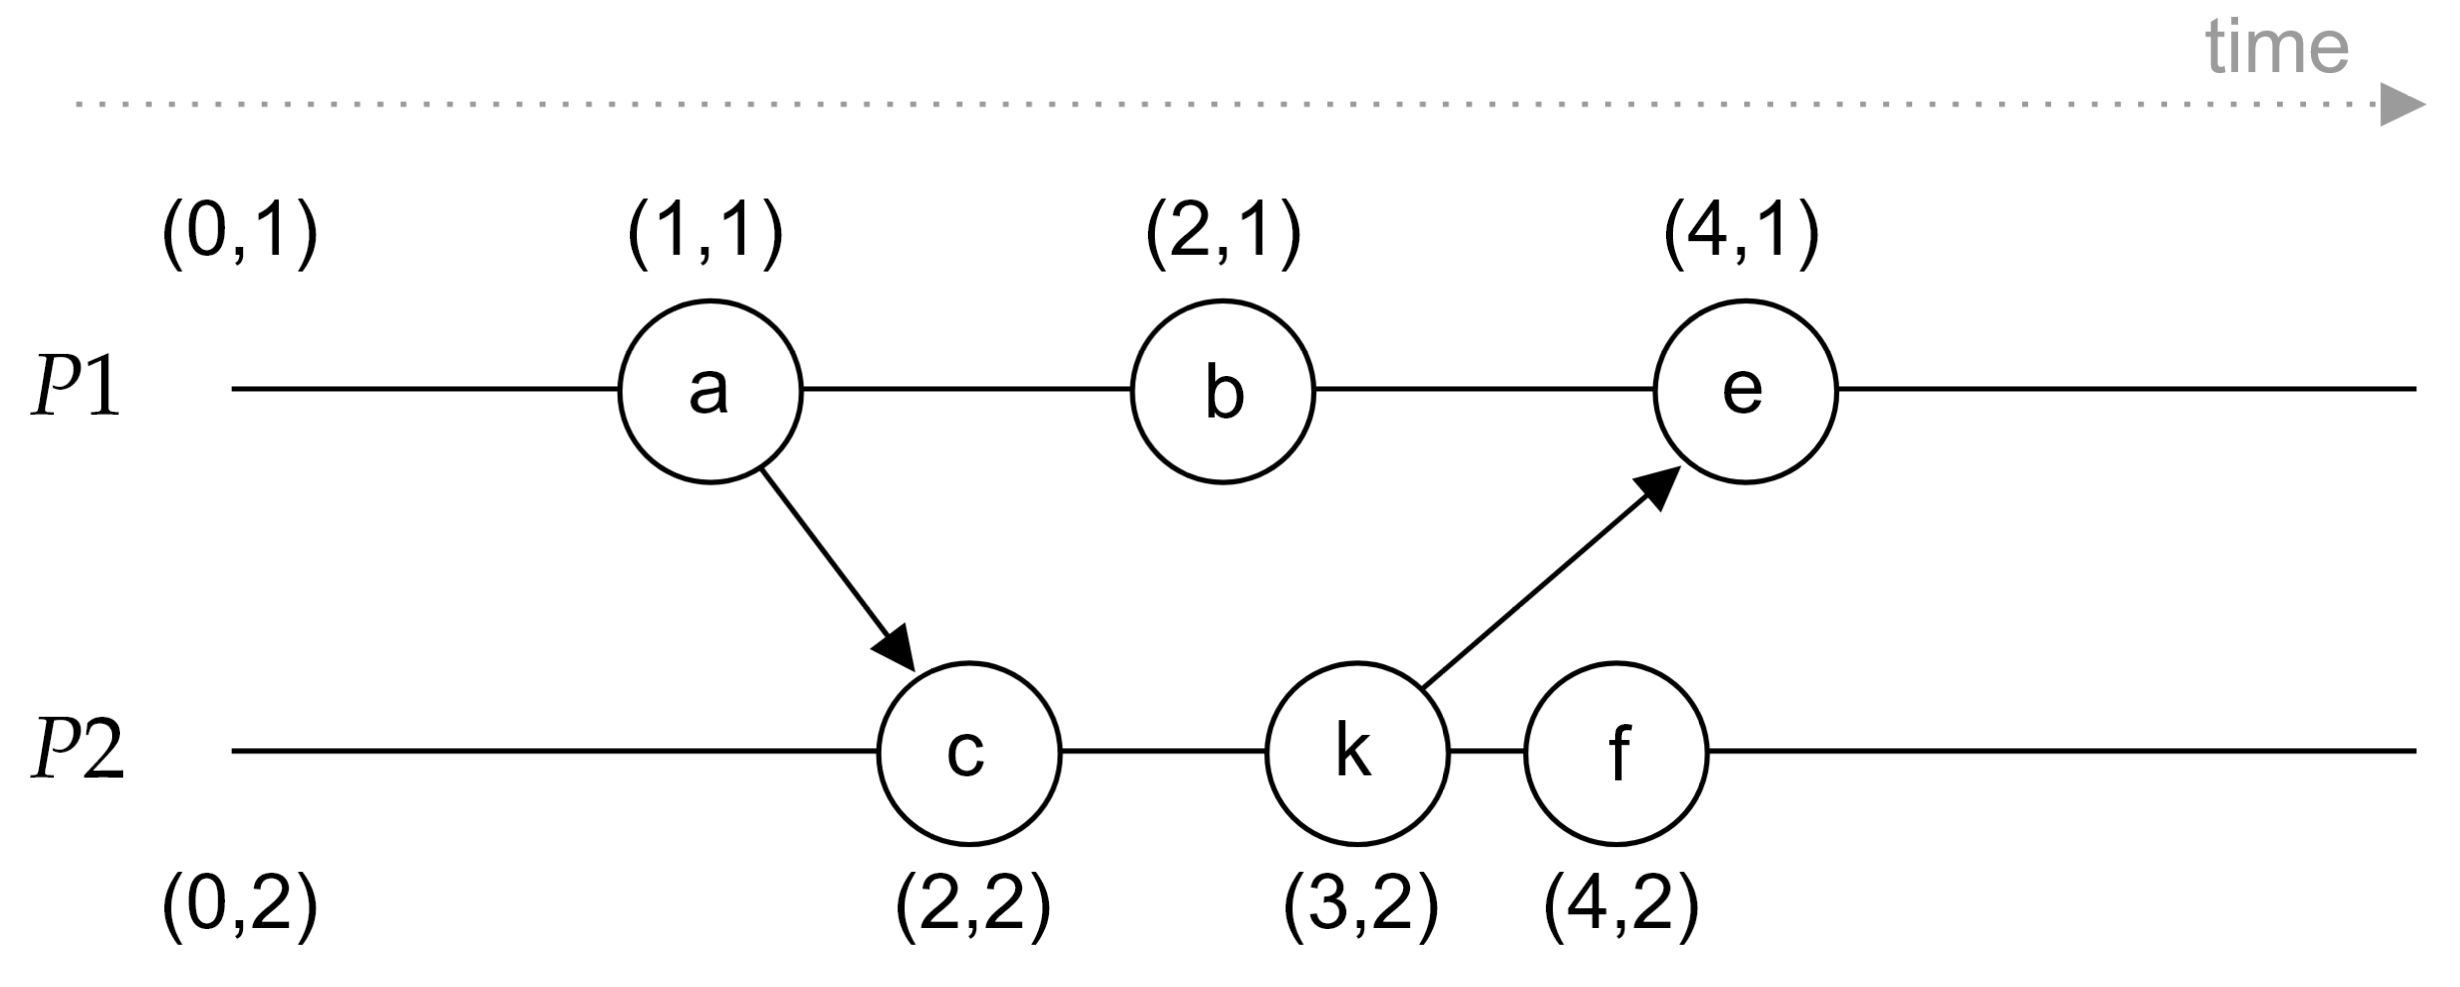
\includegraphics[width=\linewidth]{./Sections/time/lamport.png}
\end{multicols}


\newpage

\begin{multicols}{2}

\noindent
\textbf{Snapshots:} Consistent snap., captures causal dependencies, if 
$e_1 \to_r e_2$, and $e_2$ is in the snap., $e_1$ must also be present (otherwise it's inconsistent). If in the 
snap., $e_1$ sent a message to $e_2$, and $e_2$ is not in the snap., replay the message on snap. recovery.
\textbf{Chandy-Lamp.Snap:} Alg. for capturing consistent snaps. Reqs: No failures, FIFO channels, Strongly conn. graph, Single initiator.
(1) Marker sent to all out-chans., record local state. (2) On marker retrieval, block (empty) the chan. from which it came. Record local state, except for empty chans. Send marker to all out-chans.
(3) Completion, When all processes have received and sent a marker, the snapshot is complete.
(every processes' incoming channel is empty).
---\textbf{Replication}---
\textbf{Def:} Maintaining multiple copies of the same data across distinct nodes (machines), providing fault-tolerance, load-balancing, and availability.
\textbf{Active vs. Passive Rep:} Active, client sends reqs. to all replicas, must process in FIFO order. Passive, client sends reqs. to one replica (primary), which propagates to others (backups).
\textbf{State vs. Req. Rep:} State Rep., forwards the entire state to backups. Request Rep., forwards individual reqs. to backups.
\textbf{Primary Commit:} Client$\to$Primary$\to$Backups$\to$Primary$\to$Client (Commit Point).
\textbf{Arbitrary Serv. (CFG):} The Configuration Service Provider (CFG) ensures a controlled \textbf{failover} (switching to backups) in the event of a primary failure.
\textbf{Chain Rep:} An ordered chain of $s_n$ replicas, writes propagate from $s_1$ to $s_n$, where $s_n$ reports back to the client. Reads speak directly with $s_n$. For any failover, the next adjacent successor takes over.
---\textbf{Consensus}---
\pagebreak
\end{multicols}
